\appendix

\fancyhead[LE]{\tiny  \scriptsize{Annexe}}
\fancyhead[RE]{\tiny  \scriptsize{Annexe}}

{\Large\textbf{{Annexe A: Demande de temps de calcul DARI}}}\\

\phantomsection
\addcontentsline{toc}{chapter}{Annexe A: Demande de temps de calcul DARI}


\begin{figure}
\label{annexea}
\end{figure}
\begin{center}
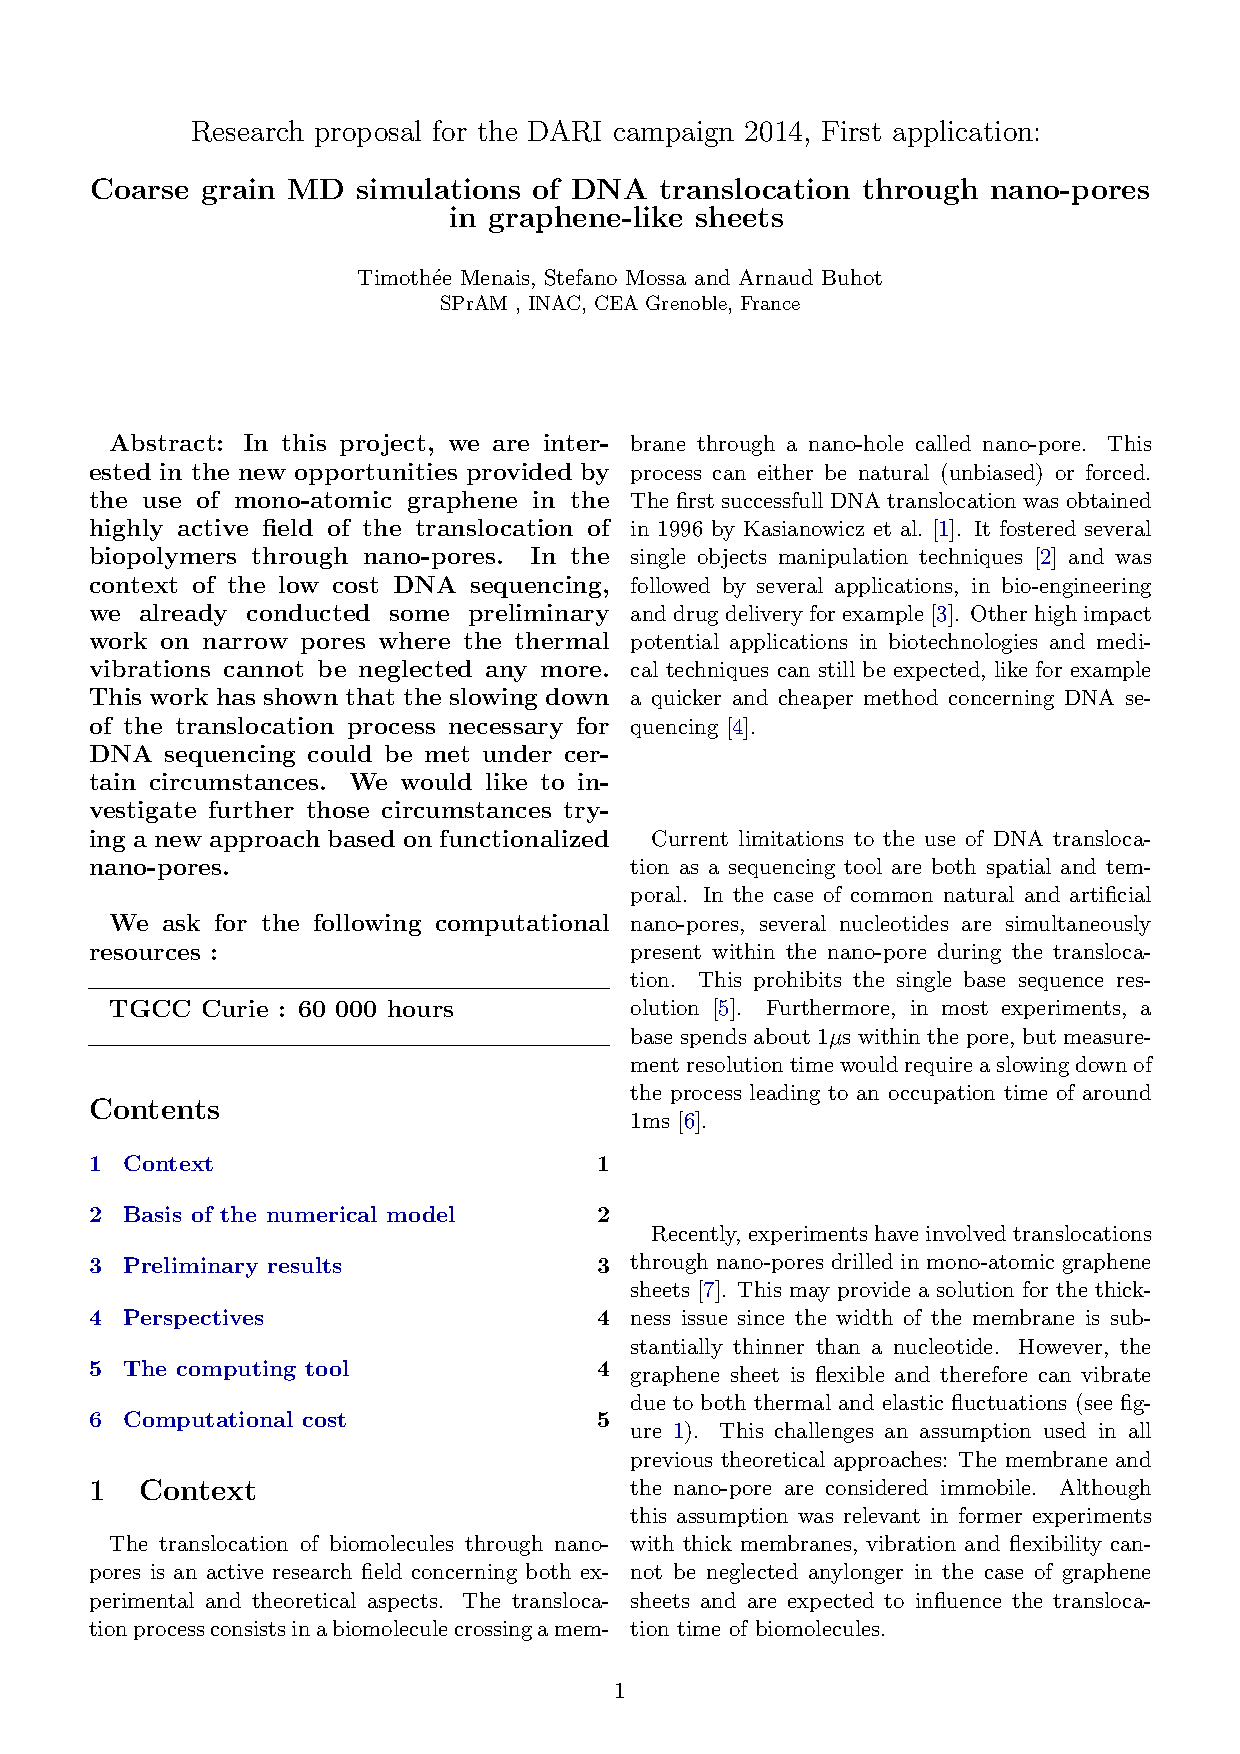
\includegraphics[width=1\textwidth , page= 1]{dari_menais_mossa_buhot.pdf}

\end{center}

\begin{center}
\includegraphics[width=1\textwidth , page= 2]{dari_menais_mossa_buhot.pdf}
\newpage
\includegraphics[width=1\textwidth , page= 3]{dari_menais_mossa_buhot.pdf}
\newpage
\includegraphics[width=1\textwidth , page= 4]{dari_menais_mossa_buhot.pdf}
\newpage
\includegraphics[width=1\textwidth , page= 5]{dari_menais_mossa_buhot.pdf}
\newpage
\includegraphics[width=1\textwidth , page= 6]{dari_menais_mossa_buhot.pdf}



\end{center}
\newpage

\verbatiminput{avisdari.txt}

\newpage

{\Large\textbf{{Annexe B: Liste des grains pour LAMMPS}}}\\

\phantomsection
\addcontentsline{toc}{chapter}{Annexe B: Liste des grains pour LAMMPS}

\begin{figure}
\label{annexeb}
\end{figure}
\verbatiminput{docgrains.txt}
\newpage

{\Large\textbf{{Annexe C: Instructions de simulation pour LAMMPS}}}\\

\phantomsection
\addcontentsline{toc}{chapter}{Annexe C: Instructions de simulation pour LAMMPS}


\begin{figure}
\label{annexec}
\end{figure}

\VerbatimInput{inputlammps.txt}



\newpage

{\Large\textbf{{Annexe D: Post-traitement}}}\\

\phantomsection
\addcontentsline{toc}{chapter}{Annexe D: Post-traitement}

\begin{figure}
\label{annexed}
\end{figure}


Lammps cré des fichiers avec des données brutes, il incombe ensuite à l'utilisateur de traiter ces données. Il a donc été nécessaire de développer des outils de traitements pour traiter ces données (rayon de giration, distance bout-à-bout, temps de translocation ...). Voici un exemple de programme écrit en language C qui permet de traiter les distributions en prenant en entrée un fichier contenant une liste brute de valeurs dont il faut extraire la distribution (ce programme fonctionne correctement avec la version 4.6 de gcc, les versions ultérieures compilent mais le programme génère des erreurs de segmentation). Nous avons également utilisé des outils écrits en C pour générer l'entrée des grains pour LAMMPS ( \hyperref[annexeb]{voir annexe B}). Les données traitées sont ensuite tracées avec Gnuplot.


\lstinputlisting[language=C]{indhisto.c}

\newpage
\thispagestyle{empty}
